\section{Франкенвордические неформологизмы}

Ужачно = удачно + ужасно --- ужасно удачно\\

\emph{Аналогично:} уржачно\\

Бабаня --- \emph{ну тут всё ясно, а вот следующее --- это ещё одно слово с 2-мя буквами ё:} Тётёля

\begin{figure}[ht!]
    \centering
    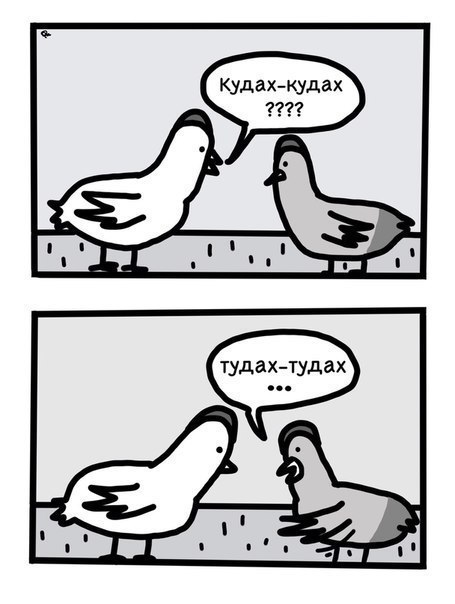
\includegraphics[width=0.6\textwidth]{tudakh}
    \caption{Alice, stop using drugs!}
\end{figure}

Идея: написать маленький рассказ из набора фраз на одну букву.\\
Главное условие: не меньше 3-х слов подряд должны быть на одну букву.

\subsection{Как заставить всех людей строить странные предложения и не стать психом}
\emph{Собственно весь "рассказ" --- это просто диалог двух обычных квазисреднестатистических людей, что является реализацией ещё одной идеи по попутному написанию литературных творений в любой наперёд заданной форме.}


\begin{itemize}
    \item[---] \emph{Я прочувствовал дух однобуквенного высказывания:}\\
    Василий Васильевич Васильев всё время валял вал\\
  --- Всё валяешь вал?\\
  --- Валяю вал\\
  --- Вандал! Варварство! Ватман!\\
  --- Ватман?\\
  --- Вероломство!\\
  Вдохновленный вандал всё валял, валял... Великолепно валял вал.
  \item[---] \emph{Вы вдохновенно ввалились в...}
  \item[---] \emph{...высказывание?}
  \item[---] \emph{Возможно.}
  \item[---] \emph{Вероятно вы верно вещаете.}
  \item[---] \emph{Ворчанием воздержитесь воздавать возведённое великолепие.}
  \item[---] \emph{"Великолепное ворчание всё время воздаёт величественную возню!"\\
Великий Воитель}
  \item[---] \emph{Вычурно вы выводите все ваши высказывания, владыка!}
  \item[---] \emph{Владею, верую, воздаю!}
   \item[---] \emph{Вмиг вмешиваете вменяемость в виртуально вывитую вещь.}
  \item[---] \emph{Виртуозно и вычурно вывернул!}
  \item[---] \emph{Наитивно навыком научились науськивать наши недра неких надумок.}
  \item[---] \emph{Адски азартно аплодирую!}
  \item[---] \emph{Да, довольно дельно думать научился на наших беседах без больших затрат за звено времени возымевшимся в своём распоряжении}
  \item[---] \emph{Дык, договорились делать данный диалог в выбранной высказывательной форме.}
  \item[---] \emph{Хорошо хоть хочу делать данный диалог.}
  \item[---] \emph{Этот эдакий энтузиазм иссякнуть или исчезнуть вполне внезапно возымеет ---
  надо наибольшее напряжение проявить при проектировании фантазируемых фурорных фраз.}
  \item[---] \emph{Очень Ожегова освежить снова следует сейчас. 
Коль когда костноязычно говоришь --- голова гудит}
  \item[---] \emph{По простецкой по причине\\
                  Коль когда костноязычишь\\
                  Говоришь гундёж гремучий\\
                  Ты теперь тут получай}
  \item[---] \emph{[полубелый стих]\\
  Трудно трутню трюизмами\\
Изысканные измышления изваять.\\
Посему повелеваем вам\\
Книжки купленны читать}
  \item[---] \emph{Загнуть заросли загубленных\\
Мыслей мешает мука моя:\\
Придумки повес пришлашённых\\
Расхоже расценила моя семья}
  \item[---] \emph{Туманно тучи толпятся в ночи\\
Ты тоже теперь его не ищи\\
Закинул зелёную зарисовку подальше\\
Не будет не будет теперь всё иначе}\\
\emph{\anttf{на этом месте мы раскрыли причину того, почему в песнях такая муть встречается. 
Мы раскрыли их зловещий план! --- Теперь мы гребём бабло! и выбрали девиз для мёртвой сосны}}
  \item[---] \emph{\anttf{Тут просто открыл словарь и читаю слова на одной стр:}}\\
             \emph{Дубильщик дубасит дрянной дубиной дрябоый дуализм дублируя дублоны дружинника...}
  \item[---] \emph{Пошёл поток прекрасных новых неформальных неологизмов!}
\end{itemize}

\framebox[0.9\textwidth][c]{
  Здесь могла быть ваша реклама, но нет!
}
